\chapter{Methods}
\label{chapter:methods}
\section{Dataset}
The dataset was created by Dr. Tichy and his team using the Computer Vision Annotation Tool (CVAT). It has been extended and improved multiple times over the course of this work, and there is still ongoing work. At the time of writing this report, it consisted of 2599 bitewing X-ray images with 4575 annotations of tooth decay. Out of those, there are 890 images without any decay. The distribution of dental caries per image is depicted in the figure \ref{fig:hist_caries_per_img}. For clarity reasons, we omitted 6 images that contained more than 10 caries. From the histogram on the figure \ref{fig:hist_caries_dim}, we observe that most of the caries have dimensions between 10 and 75 pixels. However, there are outliers as big as 380 pixels per dimension. This diversity is increasing the difficulty of the task.

We used the COCO data-format to store data, and used the format during the whole time only with rare exceptions when custom data-format was needed. During the experiments, we used the 70:15:15 split into training, validation and test dataset.
\begin{figure}
    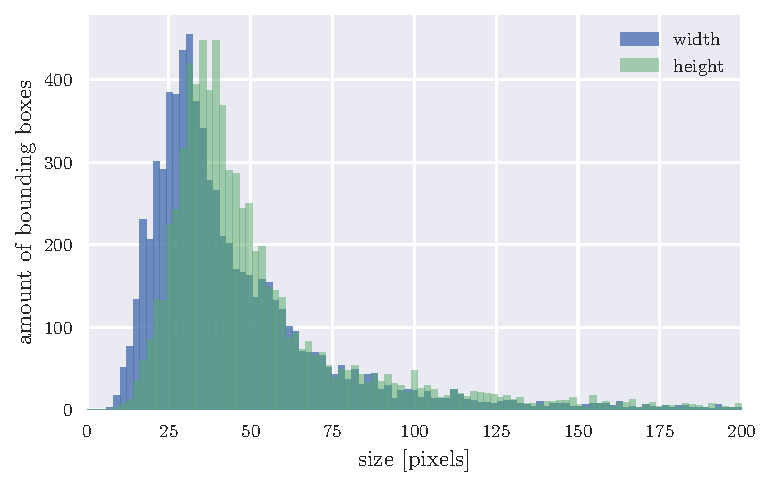
\includegraphics[width = \linewidth]{images/dataset_histogram.pdf}
    \caption{Histogram of bonding boxes dimensions in the dataset}
    \label{fig:hist_caries_dim}
\end{figure}

\begin{figure}
    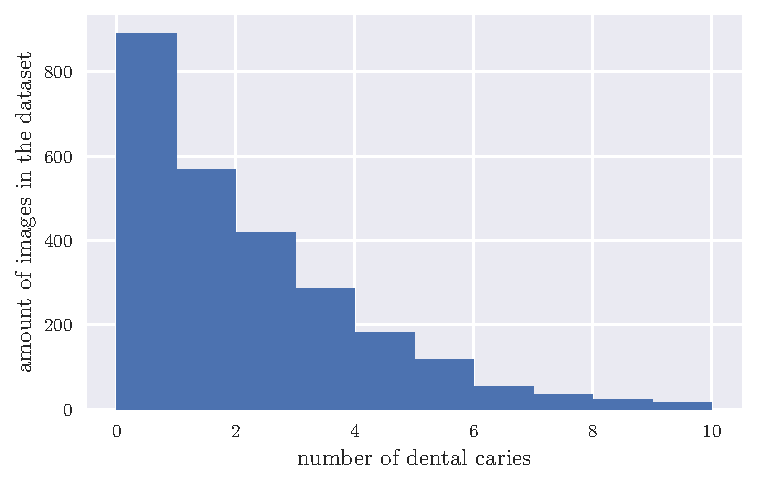
\includegraphics[width=\linewidth]{images/caries_histogram.pdf}
    \caption{Histogram of the amount of dental caries per image}
    \label{fig:hist_caries_per_img}
\end{figure}
\subsubsection{Image augmentations}
The image was augmented by a single pipeline that applied the following transformations with corresponding probabilities p.
\begin{itemize}
    \item Normalize by substracting the mean of the dataset and dividing by standard deviation of the dataset, $p=1$
    \item Resize and pad to $1024\times1024$, $p=1$
    \item Horizontal flip, $p=0.5$
    \item Vertical flip, $p=0.5$
    \item Rotation, $p=0.3$, rotation limit$=10^{\circ}$
    \item Translation, $p=0.5$, translation limit$=10\%$ of the image size
    \item Gaussian blur flip, $p=0.3$, kernel size from 7 to 31
    \item Gamma correction, $p=0.3$, $\gamma$ in range from 0.6 to 1.4
\end{itemize}

The result of those augmentations can be seen in the appendix \ref{appendix:img_transformations}.
\subsubsection{Computing power}
All the computations were realized on the CMP cluster, which consists of multiple GPU nodes. The experiments were conducted on the boruvka and zorn machines. Both of them have 32 CPU cores, 256GB of RAM memory and 8 NVIDIA GeForce GTX 1080-ti graphics cards with 12GB of dedicated memory.

\subsection{Neural network models}
\subsubsection{YOLOv5}
The YOLOv5 architecture was used with the 5l6 backbone. That is the large option from 6-th generation of the backbone architectures. When experimenting with YOLOv5 we used a batch-size of 3, which was the maximal size able to fit into the GPU memory.
\subsubsection{EfficientDet}
We used the EfficientDet-D4, because it was proposed as the optimal-efficiency architecture to use for image size of 1024 pixels \cite{Tan2019}. Even though there are 3 bigger backbones available, the batch size has to be 1 for the network to fit into the GPU.

\subsubsection{Optimizers}
The Adam optimizer was used during all experiments. The parameters $\beta_1, \beta_2$ were set to 0.9 and 0.999 and weight decay was chosen to be $1e^{-6}$. Since we were not able to fit a reasonably big batch-size into the GPU, the optimization step was performed every 4  steps forward. This should emulate bigger batch-size and increase the chance of finding global optimization minima.
\subsubsection{Learning rate}
The initial value of the learning rate was set to $1e^{-5}$ and reduced on plateau learning rate scheduler was used. The monitored value by the scheduler was validation loss and learning rate decreased by the factor of 5, when the imporovement of the loss stalled for 5 epochs.
\subsubsection{Termination condition}
The training was halted when the validation error did not decrease over the course of 10 epochs, but not earlier than after 50 epochs.


